%!TEX root = ../thesis.tex
\chapter{Background}
\label{ch:background}

\section{Hexapods}
Hexapods are a class of robots featuring 6 legs, inspired by the locomotion of insects and arachnids.
Over millions of years of evolution these organisms developed efficient strategies to navigate challenging terrain, making them a rich source of inspiration for robotics.
By emulating the biomechanics and behavior of insects, researchers and engineers aim to create versatile and robust robotic systems capable of navigating challenging terrain.

Most commonly, each leg of a hexapod typically consists of 3 segments named coxa, femur and tibia, equivalent to their biological counterparts.
The individual segments are connected by 3 2-DoF(degrees of freedom) joints, each actuated by an electric servo motor.
The first joint, hereafter named \textalpha-joint, connects the coxa to the thorax(body) and moves in parallel to the ground, thus being responsible for the longitudinal placement of each leg.
Coxa and femur are connected by the \textbeta-joint, while the femur and tibia are connected by the \textgamma-joint. 
These joints move orthogonal to the movement plane of the \textalpha-joint. Together, they are responsible for the lateral positioning of each leg.
The nomenclature we use use in thsis thesis to label the joints and leg segments was adopted from the works of Schilling, Cruse, Hoinville et. al. \parencite{schilling2013walknet, HeterarchicalArchitectureSchilling}.

\begin{figure}[h]
	\centerline{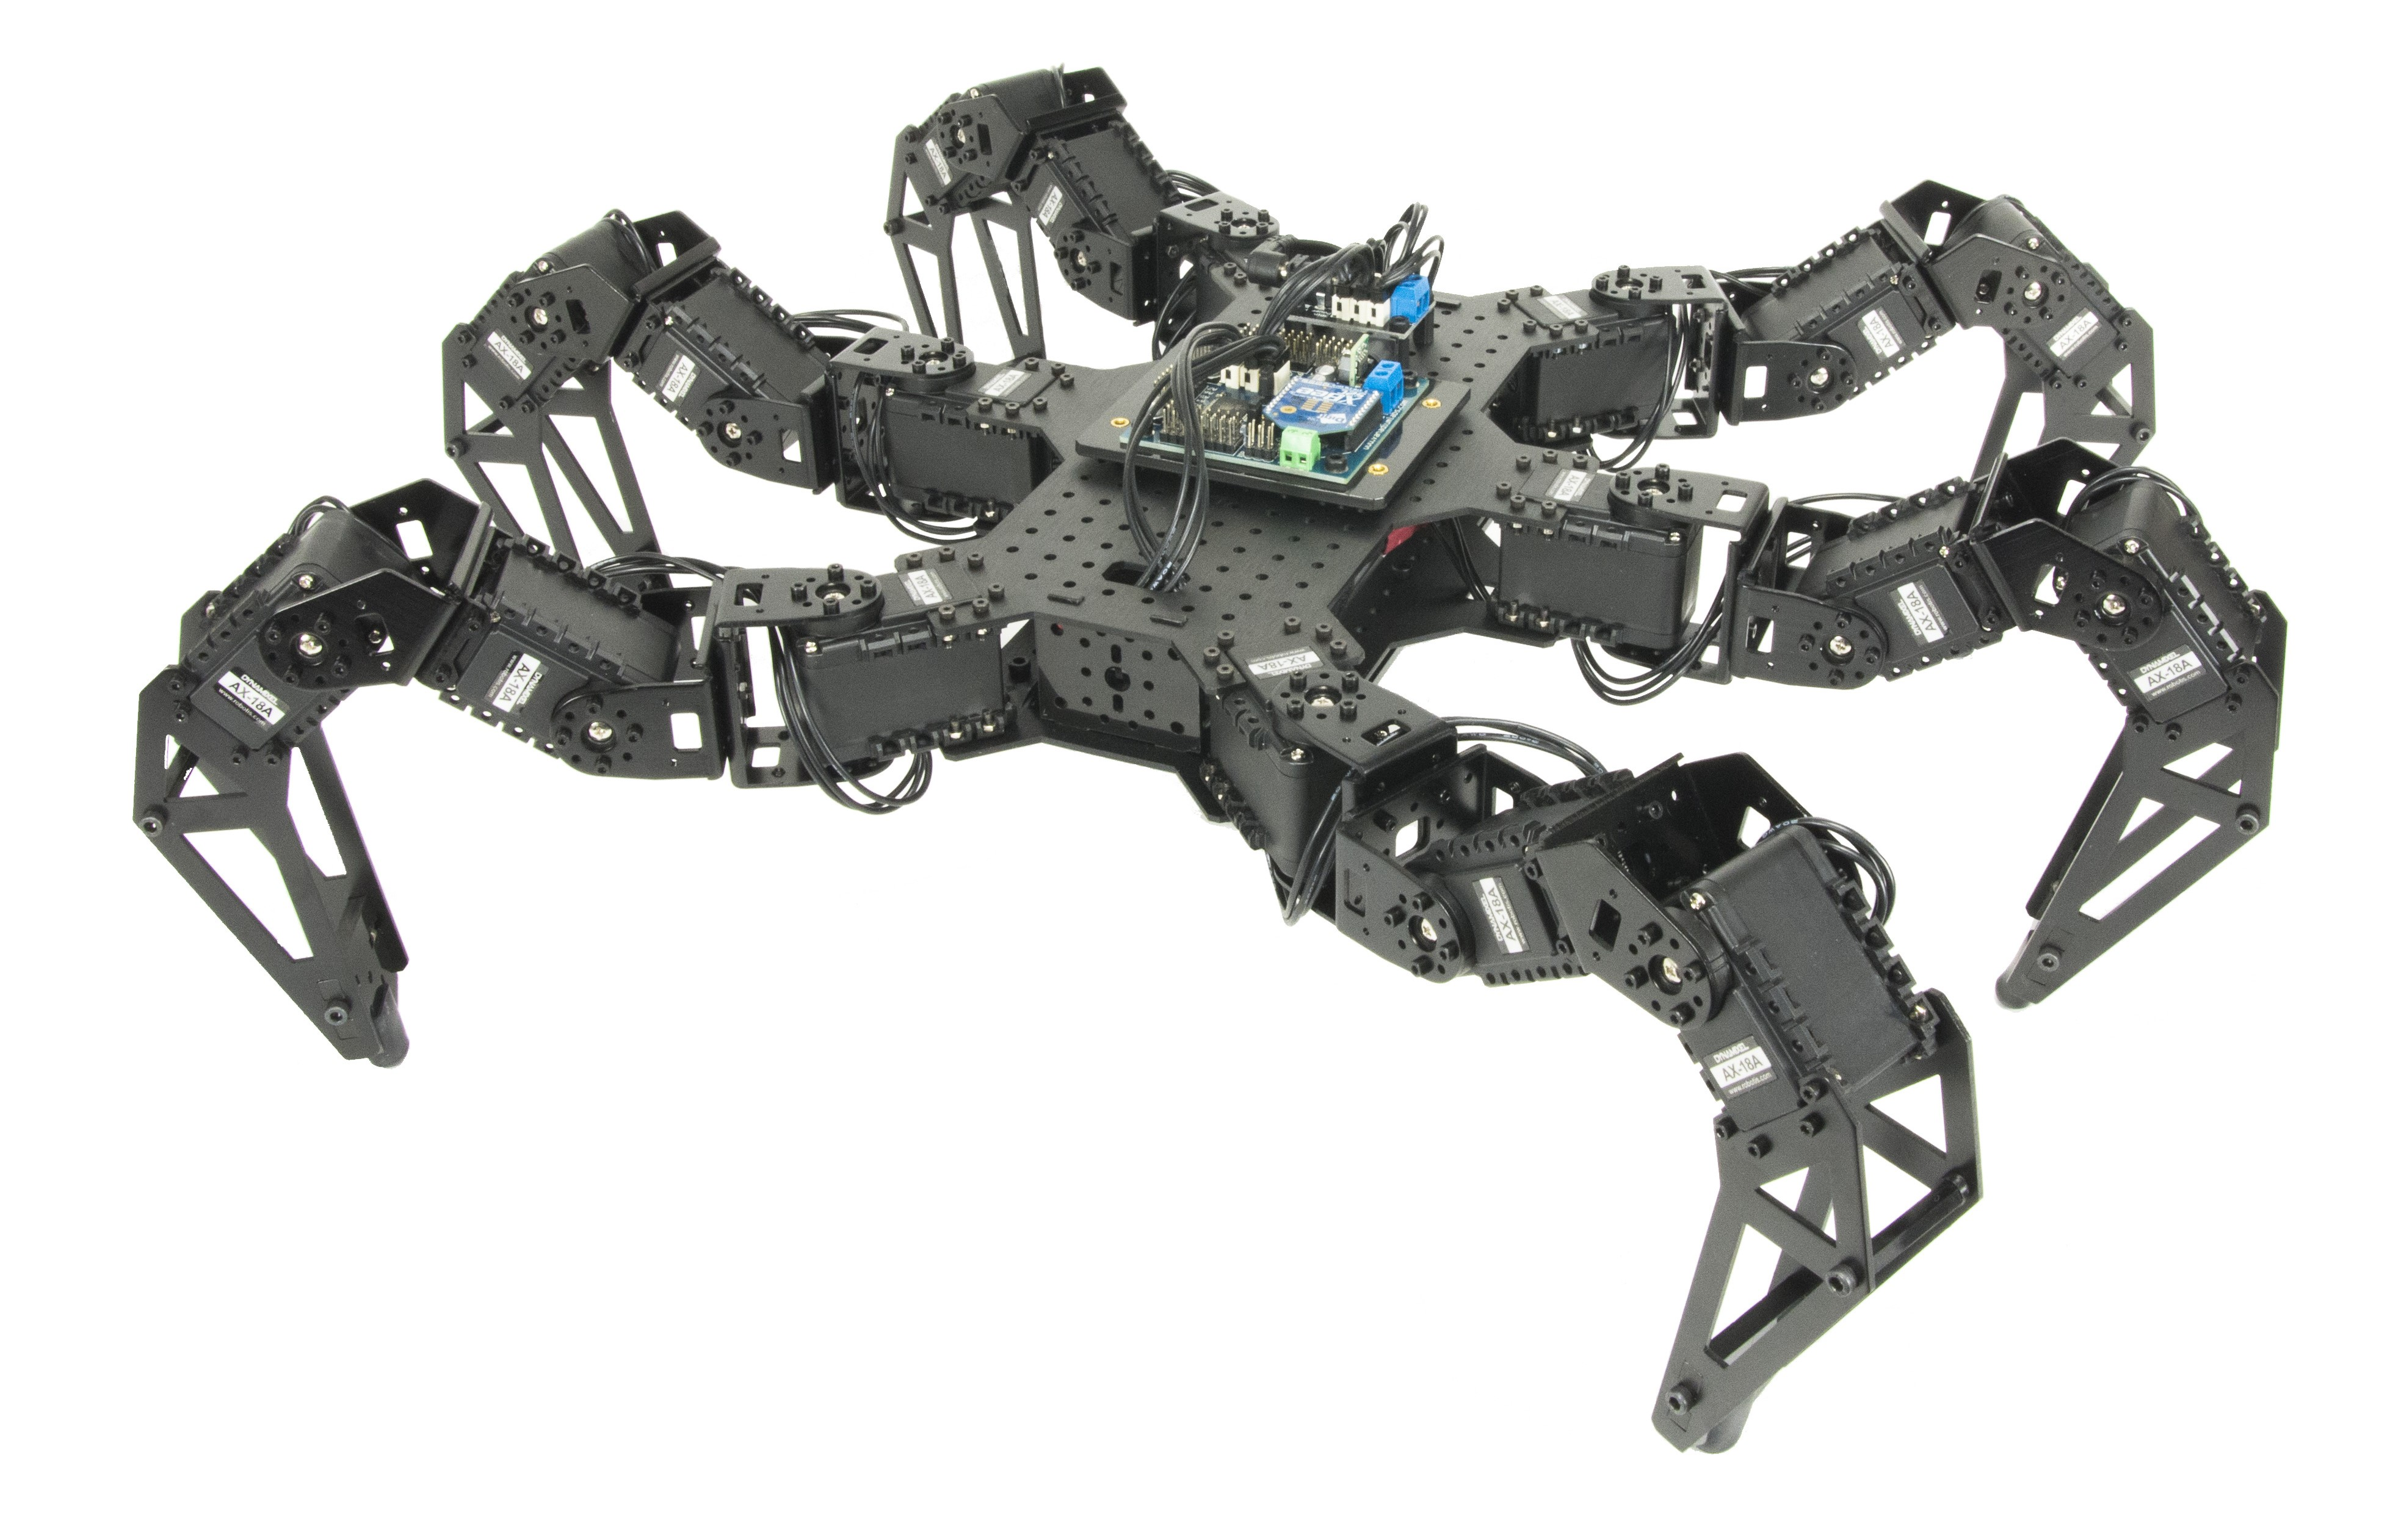
\includegraphics[scale=0.04]{phantomX_III_overview}}
	\caption{PhantomX MKIII hexapod, predecessor of MKIV used here [\cite{PhantomX_MKIII}]}
	\label{figure: PhantomX MKIII}
\end{figure}

\todo{"Gait Self-learning for Damaged Robots Combining Bionic Inspiration and Deep Reinforcement Learning" for parameters of hexapod}

\todo{Maybe add image of stick insect}

\todo{CITATIONS}

\section{MATLAB}
\hiddensubsection{Simulink}
\textit{Simulink\textsuperscript{\textregistered}} is a \textit{MATLAB\textsuperscript{\textregistered}}-based graphical block-diagramming tool developed by the company \textit{MathWorks\textsuperscript{\textregistered}}. 
It is a widely used tool which plays a crucial role in various engineering and research disciplines.
It provides the user with a versatile platform to design, simulate and analyze complex dynamic systems.

Simulink offers an expansive library of predefined blocks that represent different components and behaviors.
The user connects these blocks with so called signal lines to transport data between them.
Blocks transform the data provided by the inputs and output the transformed data to other blocks connected downstream.
Their behavior can be discrete, like a switch which activates when a signal is high, or represent continuous functions such as integrals.

An arrangement of blocks can be encapsulated into a subsystem, thus creating different levels of abstraction.
To enable easy reuse, subsystems can be placed in custom libraries.
If a library object gets updated, each linked copy of this subsystem receives the update as well, preventing the user from having to edit each copy themselves.
At any step in the development process, a model can be simulated and analyzed.
The value of any signal lines can be plotted and the simulation can be slowed down.

\begin{figure}[h]
	\centerline{\includesvg[scale=0.8]{Simulink/BouncingBallExample_Simulink.svg}}
	\caption{Simulink model of a bouncing ball created using standard library blocks.}
	\label{figure: Simulink Bouncing Ball Example}
\end{figure}

\hiddensubsection{Simscape}
\textit{Simscape\textsuperscript{\texttrademark}} is a block library developed by \textit{MathWorks\textsuperscript{\textregistered}} enabling the modeling of physical systems within the Simulink environment.
Utilizing this library it is possible model and simulate systems such as electric circuits, hydraulics or classical mechanics all within a unified simulation environment.
Simscape offers a large variety of predefined components like resistors, capacitors, springs, dampers and more.
To understand the model we developed, the mechanical components are of the most interest, especially coordinate frames, transforms, joints and rigid bodies.
Coordinate frames can be attached to each other using rigid transforms or joints.
Joints allow for different degrees of freedom between two frames, depending on what constraints should be imposed on the system.
Two frames connected with a joint are named base and follower frame.
When the joint is actuated, the follower frame moves relative to the base frame\parencite{thilderkvist2015motion}.
Rigid transforms translate or rotate coordinate frames without allowing for any degree of freedom.
Rigid bodies can be connected to the predefined coordinate frames, providing shape, mass and inertia to the system.
If the user requires a component which is not yet represented by any block in the libraries, Simscape also offers a MATLAB based language to enable text-based development of custom components.
\todo{Weiter ausführen; mehr Details, z.B. über Gelenke(Sensorik, Aktuation, etc.)}
\todo{CITATIONS}

\begin{figure}[h]
	\centering
	\centerline{\includesvg[scale=1.0]{Simulink/BouncingBallExample_Simscape.svg}}
	\
	\caption{Simulink model of the same system as in Fig. \ref{figure: Simulink Bouncing Ball Example} but created solely with Simscape blocks.}
	\label{figure: Simscape Bouncing Ball Example}
\end{figure}

\section{Insect Locomotion}

\begin{figure}[h]
	\centerline{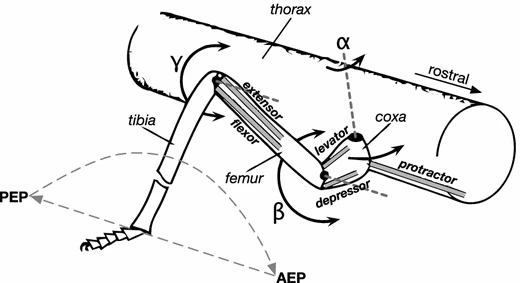
\includegraphics[scale=0.5]{morphologyOfStickInsect_sketch}}
	\caption{Morphologic drawing of a stick insect leg (\cite{schilling2013walknet} [Fig.1]).}
	\begin{footnotesize}
		Angle $\alpha$ represents the position of the thorax-coxa joint, angle $\beta$ describes the position of the coxa-femur joint and angle $\gamma$ represents the position of the femur-tibia joint.
		These joints are actuated with three pairs of muscles, protractor-retractor, levator-depressor and extensor-flexor respectively.
		Also depicted are the posterior extreme position(PEP), defined as the rearmost point of the movement cycle, and the anterior extreme position(AEP), the foremost point in the cycle.
		Dashed lines depict the swing and stance movement between PEP and AEP.
	\end{footnotesize}
	
	\label{figure: Stick insect leg}
\end{figure}

The swing-stance cycle depicted above is an essential element of an insects locomotion.
When in stance phase, the leg is in contact with the ground and bears a partial load of the insects weight.
The leg moves backwards, relative to the body, from AEP to PEP. During this phase the leg pushes the insect forward.
During the swing phase the leg is lifted of the ground and moved form PEP to AEP in an arch.
The stance phase is responsible for moving the insect forward until reaching the PEP, when the swing phase is needed to reposition the leg at the AEP to start the cycle again.
The complete cycle can be described as a pushing phase(stance) and a repositioning phase(swing).

\todo{CITATIONS}
\todo{Expand}


\section{Inverse Kinematics}
Inverse Kinematics(IK) is a term predominately used in robotics and computer graphics.
It describes the process of calculating the joint angles required to place the end of a kinematic chain, such as a robotic manipulator, at a given position and orientation.
There are two distinct methods how to calculate these angles, analytical and numerical.

Analytical solvers are based on trigonometric equations derived from the geometric and kinematic parameters of the manipulator arm, such as the link length, joint type and joint limits.
They provide exact solutions and can be significantly faster than iterative approximation methods.
Although very efficient and precise, the analytical approach is generally only feasible for kinematic chains with a small number of DoF.
If ,for the kinematic chain, the number of DoF is greater than the number of DoF of the end-effector, then there exist infinite solutions for a given pose.\todo{SOURCE ?}
These kinds of systems potentially lack closed-form expressions for a solution, which makes deriving analytical solutions infeasible if not impossible.


Numerical solvers use iterate approaches to approximate the joint angles and converge towards a solution over several iterations of their algorithm.
At the start of the process, this type of solver begins with an initial guess
This guess can be based on the manipulators geometry, joint limits, previously obtained solutions, or other heuristics.
Using the estimated joint angles, the would-be position of the end-effector is calculated(forward kinematics) and the error between the desired pose and the currently obtained pose is determined.
Based on this error, the joint angles are adjusted with the goal of reducing the error and bringing the end-effector closer to the desired pose.
This process is repeated until the error meets the predefined tolerances.
The joint angles calculated during the final iteration are then considered a solution to the problem.
Although the basic principle of error-minimization is always present in the algorithm, the exact process of minimization is much more complex than described here and there exist numerous different techniques on how to achieve this goal.
Numerical solvers can be applied to a wide variety of inverse kinematics problems and are not limited by the number of DoF like analytical solvers.
Due to their iterative nature numerical solvers are generally more computationally expensive, given the same problem, than their analytical counterparts.

Both inverse kinematics methods are used extensively in industry and research, depending on the specific project and its requirements.
\todo{CITATIONS}
\todo{Describe filter coefficient N}




\section{PID Controller}
A \textbf{P}roportional-\textbf{I}ntegral-\textbf{D}erivative(PID) controller is a widely used feedback control system.
As such, it aims to regulate a control variable to a desired setpoint by adjusting its output according to the currently measured process variable.
In most cases this process variable corresponds to a real world variable such as the speed of a motor, the liquid-level inside a tank or the temperature of a furnace.
It uses three terms, a proportional, integral and derivative term, to compute the controlled output based on the error between the setpoint and current process variable.
Focusing on digital PID controllers, the process of error calculation and control variable adjustment is done at a discrete, fixed rate and is also referred to as a time step.
There also exist implementations of this control loop type using analog electronics which generate a continuous control signal, but these are of no concern for the content of this thesis.
In the following section we will describe the operation of a PID controller in detail:

\begin{figure}[h]
	\centerline{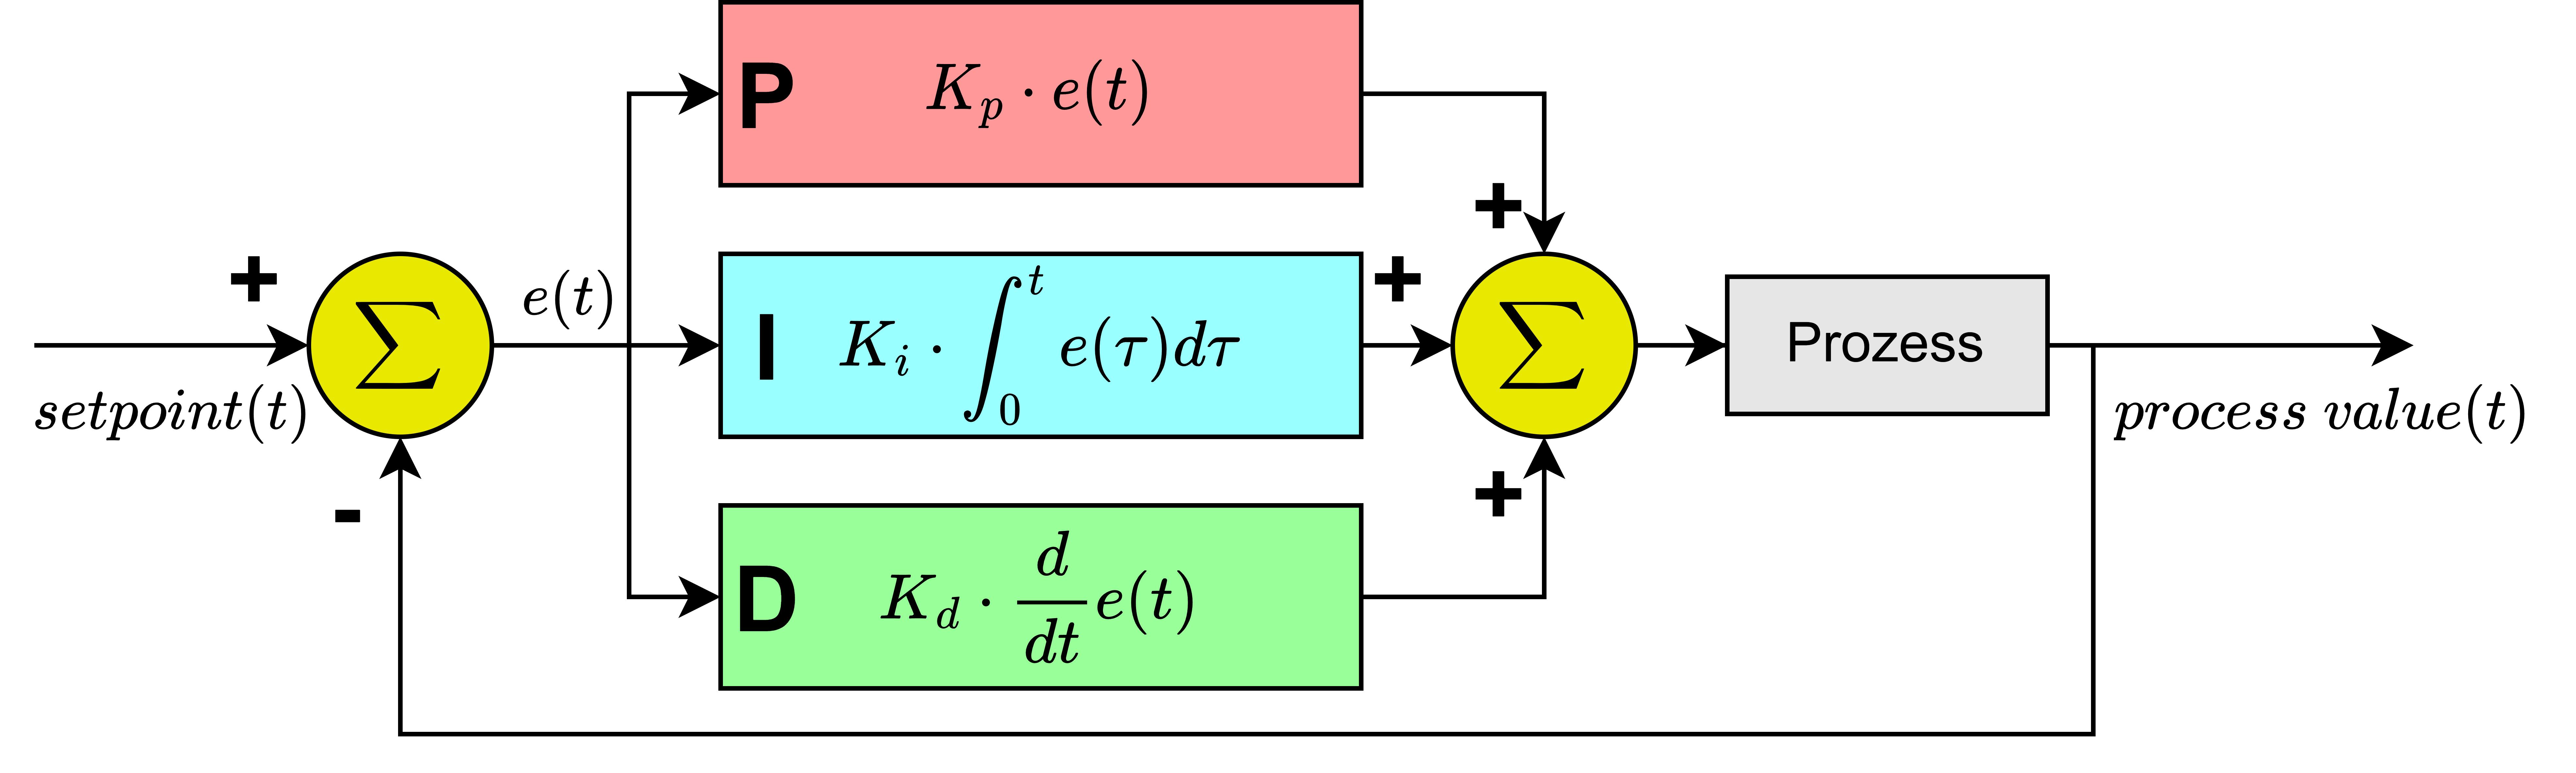
\includegraphics[scale=0.05]{PID_Controller}}
	\caption{Illustration of a PID Controller}
	\label{figure: PID Controller}
\end{figure}
\todo{Change d and dt to /partial in pid graphic}

At each time step the controller first calculates the error between its setpoint and the currently measured process variable: 
\[
	Error(t) = setpoint - process\ variable(t)
.\]
After the error is determined, the controller then determines the proportional, integral and derivative term based on this error.

The proportional term $P(t)$ is calculated by multiplying the error by a constant factor, the so called proportional gain $K_p$.
This term contributes to the control output, as its name suggests, proportional to the magnitude of the error.
$P(t)$ is given by:
\[
	P(t) = K_p \cdot Error(t)
.\]
The integral term $I(t)$ takes the sum of past errors into account to address any long term bias/ constant error contained inside of the controlled system.
It is able to eliminate long-term errors that can not be accounted for by $P(t)$.
The term is calculated by integrating the error over time and multiplying it with the integral gain $K_i$.
$I(t)$ is given by:
\[
	I(t) = K_i \cdot \int_{0}^{t} Error(\tau) \,d\tau
.\]
The derivative term $D(t)$ anticipates the errors future behavior by determining its rate of change.
It prevents the controller from overshooting and oscillating by dampening the control response.
$D(t)$ is calculated by multiplying the errors rate of change with the constant derivative gain $K_d$.
It is given by:
\[
	D(t) = K_d \cdot \frac{\partial}{\partial t}(Error(t))
.\]
The final output of the controller at time $t$ is then given by the sum of all three terms:
\[
	Control\ Output(t) = P(t) + I(t) + D(t)
.\]
The calculated control output is fed into the controlled system or process and the PID controller calculates the next control value.

In real-world applications the derivative term is almost never implemented as a pure derivative as it would be extremely sensitive to noise.
Instead, a so called filter coefficient $N$ is added to modify the derivative.
The modified derivative term is given by:

\[
...
\]
The term acts as a first-order, low pass filter, meaning frequencies in the signal above a specific limit are ignored.
It thus behaves like a derivative up to a given cutoff frequency given by: \todo{cutoff frequency}.

The performance of a PID controller greatly depends on the values of its parameters $K_p$, $K_i$ and $K_d$.
To achieve desired results like fast response times and minimal overshooting or oscillations, these parameters have to be carefully tuned. 
This tuning process can be done manually by trial-and-error or methodically with a tuning algorithm.

To conclude, a PID controller continuously repeats the process of error calculation and adjustment, thus forming a closed-loop system which aims to minimize the error and approach the setpoint as close as possible.

\todo{CITATIONS}




\section{Reinforcement Learning}

Reinforcement Learning(RL), besides supervised and unsupervised learning, is one of the three major branches in the vast field of Machine Learning.The basic underlying principle of RL is to learn how a scalar reward signal can be cumulatively maximized \parencite{sutton2018reinforcement}.
In simple terms, RL focuses on training an agent(or multiple agents) to take sequences of actions in an environment as to maximize a cumulative reward.
Some of the principles used in RL are inspired by behavioral psychology, where learning is mainly driven by the consequences of the actions taken \parencite{sutton2018reinforcement, FINDAUTOR}\todo{Cite author for behavioral psych.}.

\begin{figure}[h]
	\centerline{
\includegraphics[scale=0.1]{RL_Overview}}
	\caption{The basic concept of Reinforcement Learning (\cite{weng2018bandit} [Fig.1])}
	\label{figure: RL Illustration}
\end{figure}

The agent, as seen in \ref{figure: RL Illustration}, is the entity which learns, it takes actions in the environment and receives observations and the reward signal from the environment.
An agent always acts according to its current policy.
A policy roughly defines a mapping of all perceived environmental states to actions to be taken by the agent.
It fully  describes the way a learning agent behaves at any given point(in time) in the learning process.\parencite{sutton2018reinforcement} \parencite{D. Silver Lec. 2}
The agents policy is continually updated during the learning process, always trying to improve the actions taken by the policy towards a higher expected reward.

The environment is the place in which the agent tries to improve its policy by taking actions and learning from them.
It defines the problem which the RL agent is supposed to solve by learning a policy.
The problem definition can range from robotic control tasks such as walking or autonomous driving over playing video games all the way to advertisement or news recommendations.
The environment 
Every problem for which as a reward function can be defined which accurately represents the agents performance.\todo{refactor this section}
The environment receives the actions chosen by the agent and computes the resulting environmental state and the amount of reward the agent receives for the state it is in.
It provides the reward and observations about the environment to the agent.

The RL process is repeated for every time step.

The reward function or reward signal is a scalar function which defines the goal of the reinforcement leaning problem.
At each time step, this function is evaluated and the scalar output, the reward, is sent to the agent.
The maximization of this reward is the sole objective of the agent.
Due to the reward being the only metric which defines what agent behavior is good and bad, it is important to define this function well.
If the reward function is poorly defined, the agent will perform poorly as well.
The reward function is considered part of the environment.
\parencite{sutton2018reinforcement}



\parencite{weng2018bandit}
\parencite{sutton2018reinforcement}

Model-Free vs. Model ?


\begin{definition*}
	A policy $\pi$ is a distribution over actions given states,\\
	$\pi(a|s) = \mathbb{P}(A\textsubscript{t} = a\,|\,S\textsubscript{t} = s)$
\end{definition*}
A policy fully defines an agents behavior. 
\todo{Cite David Sijlver Lec. 2}

A value function, in contrast to a reward function which immediately rewards good actions, defines what is good long term. 
Rewards only define the immediate desirability of environmental states, a value function takes into account states which are likely to follow a given state and the rewards available in those states.
A state might immediately yield a low reward, but if it is likely followed by states which yield high rewards, it can still possess a high value.
This can also be true for the opposite, a state has a high immediate reward, but is likely only followed by states which yield low rewards. Thus the state has a low value \parencite{sutton2018reinforcement}.

Some methods of solving RL problems also consider a model of the environment. This means that the approach has a way of planning ahead, such as predicting the next environmental state and reward.
Methods which use a model are called model-based, methods which explicitly only learn by trial and error model-free\parencite{sutton2018reinforcement}.

Offline vs. Online Reinforcement Learning: 
RL agents labeled as offline only learn from a fixed dataset which has been acquired before starting the training process.
The agent itself does not interact with the environment, only learning on historical data.
Online RL agents on the other side learn while actively interacting with the environment.
They decide, act and receive feedback all in real-time and learn from the consequences of their actions \parencite{schrittwieser2021online}.



Discrete vs. Continuous action space in RL learning: 
A discrete action space is used when the number of actions that can be taken is limited and known in advance. An example of such an environment would be a game of chess; each turn there is a finite number of avaiable moves.
Continuous action spaces are used, when the number of possible actions is not knowable in advance and possibly infinite\todo{Just write infinite and cite ?}, such as the movement possibilities of a robotic arm.
Because we have multiple robotic 'actuators' in this project, a continuous action space is favorable.


Markov Property: "The future is independent of the past given the present"
The current state contains all relevant information to make predictions about the future
\begin{definition*}
	State S\textsubscript{t} is \textbf{\textit{Markov}}, if and only if
	$ P(S\textsubscript{t+1} | S\textsubscript{t}) = P(S\textsubscript{t+1} | S\textsubscript{1},...,S\textsubscript{t}) $.
\end{definition*}

Markov Process:
A Markov Process is a memory-less random process, i.e. a sequence of random states S\textsubscript{1}, S\textsubscript{2},... that have the Markov property.

\begin{definition*}
	A Markov Process (or Markov Chain) is a tuple $\langle\mathcal{S,P}\rangle$ where
		\begin{itemize}
		\item $\mathcal{S}$ is a (finite) set of states that have the Markov property
		\item $\mathcal{P}$ is a state-transition probability matrix,\\
		$\mathcal{P}\textsubscript{ss'} = \mathbb{P}[S\textsubscript{t+1} = s'|S\textsubscript{t}=s] $
	\end{itemize}
\end{definition*}
\todo{Cite David Silver RL course Lec. 1-2 for everything about Markov}

Markov Decision Process(MDP):

$\rightarrow$ Hexapod locomotion can be considered a MDP, see: \parencite{ouyang2021adaptive} [p.7, 4.1]
$\rightarrow$ Try DDPG for RL, allegedly widely used in robotics \parencite{ouyang2021adaptive}


Agents applicable for continuous action spaces: 
\begin{itemize}		
	\item DDPG: Deep Deterministic Policy Gradient
	Model-free, continuous action space, actor-critic (Look at \parencite{trotta2022walking})
	\item TD3: Twin-Delayed Deep Deterministic Policy Gradient (more complex improvement to DDPG)
	Model-free, continuous action space, actor-critic
	\item PPO: Proximal Policy Optimization (more stable updates, but longer training)
	Model-free, continuous or discrete action space; policy gradient rl-method
	\item SAC: Soft Actor-Critic (more complex improvement of DDPG generating stochastic policies)
	Model-free, continuous action space, actor-critic
	\item TRPO: Trust Region Policy Optimization(more complex version of PPO, more robust for deterministic environments with fewer iterations)
\end{itemize}
\todo{Cite MATLAB}
\todo{Use image for explanation}